\documentclass[11pt,a4paper]{article}
\usepackage[utf8]{inputenc}
\usepackage{amsmath,amssymb}
\usepackage{graphicx}
\usepackage[hidelinks]{hyperref}
\usepackage{booktabs}
\usepackage{geometry}
\usepackage{caption}
\usepackage{subcaption}
\usepackage{array}
\usepackage{adjustbox}
\usepackage{float}
\geometry{margin=1in}

\title{The Modality Paradox in Autonomous LLM Engineering: Asymmetric Agent Loops and Mathematical Halting}
\author{Sanskar Jajoo \\ Neuralchemy Labs \\ \url{https://www.neuralchemy.in/} \\ \url{https://github.com/m4vic/AEOS}}
\date{}

\begin{document}
\maketitle

\begin{abstract}
As Large Language Models (LLMs) are deployed in autonomous closed-loop engineering workflows, a recurring failure mode emerges: the \textit{Autonomous Sunk-Cost Fallacy}. A monolithic agent often continues low-yield strategy edits for dozens of iterations despite negligible progress, consuming large compute budgets.

This paper focuses exclusively on that failure mode in machine learning engineering loops. We evaluate single-agent and asymmetric Reviewer$\rightarrow$Coder architectures across Tabular, Text, and Vision modalities in AEOS. We formalize Sunk-Cost Episodes (SCEs), define the Cognitive Agentic Diversity Score (CADS), and introduce the $\Omega$ Cognitive Yield Engine for mathematical stopping.

In addition to the baseline modality experiments, we run a targeted mathematical self-reflection ablation (N=36): 3 datasets $\times$ 4 architectures $\times$ 3 repeats. The ablation shows strong autonomous stopping behavior (35/36 runs halt via reviewer directive) while revealing a modality-dependent optimum: the best architecture is not globally fixed. We conclude that robust autonomous optimization requires both role asymmetry and mathematically grounded halting; the mathematical gate achieves 35/36 reviewer-issued stops while preserving near-equivalent peak accuracy, with task modality governing the persistence-efficiency tradeoff.
\end{abstract}

\section{Introduction}

The prevailing roadmap toward Artificial General Intelligence (AGI) is heavily anchored on the scaling laws of monolithic transformers. While increasing parameter sizes has yielded breakthroughs in static benchmarks, these architectures degrade significantly when deployed in closed-loop, autonomous engineering loops.

In Paper 2 (Jajoo, 2026b), we deployed 13 LLMs into the Autonomous Empirical Optimization System (AEOS) and discovered the \textbf{Autonomous Sunk-Cost Fallacy}. When a single agent begins to fail, it generates minor, mathematically insignificant hyperparameter tweaks for 50 to 100+ iterations. General-purpose models consumed upwards of 3,400 seconds trapped in Sunk-Cost Episodes (SCEs).

\begin{figure}[ht]
    \centering
    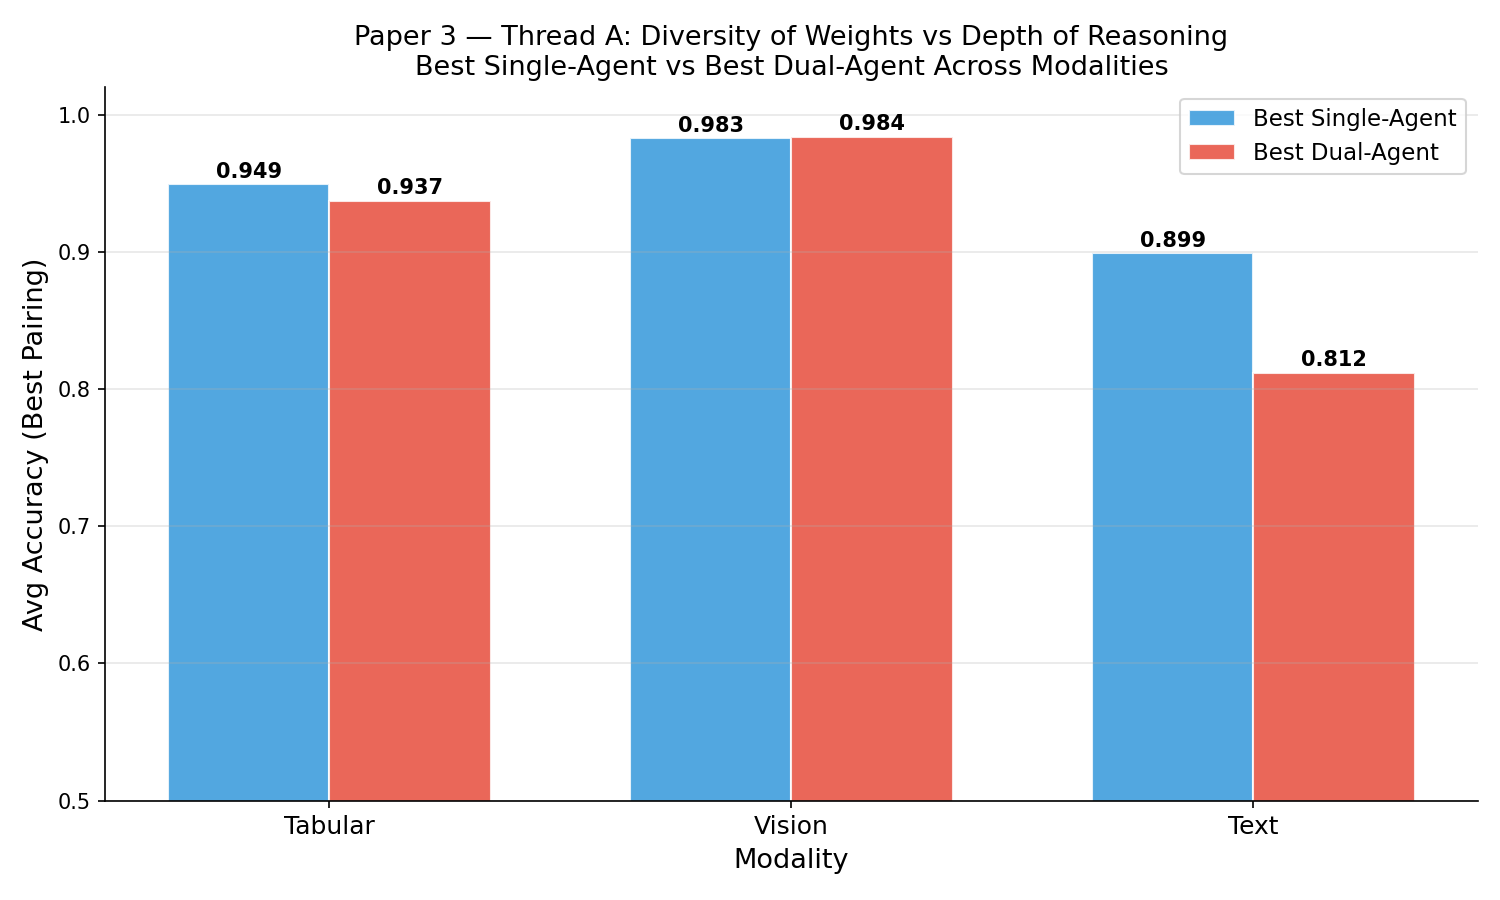
\includegraphics[width=0.8\textwidth]{figures/fig1_cross_modality_summary.png}
    \caption{Cross Modality Efficiency: Comparing the raw capability vs. efficiency of single models against asymmetric dual-agent architectures.}
    \label{fig:cross_modality}
\end{figure}

\begin{figure}[ht]
    \centering
    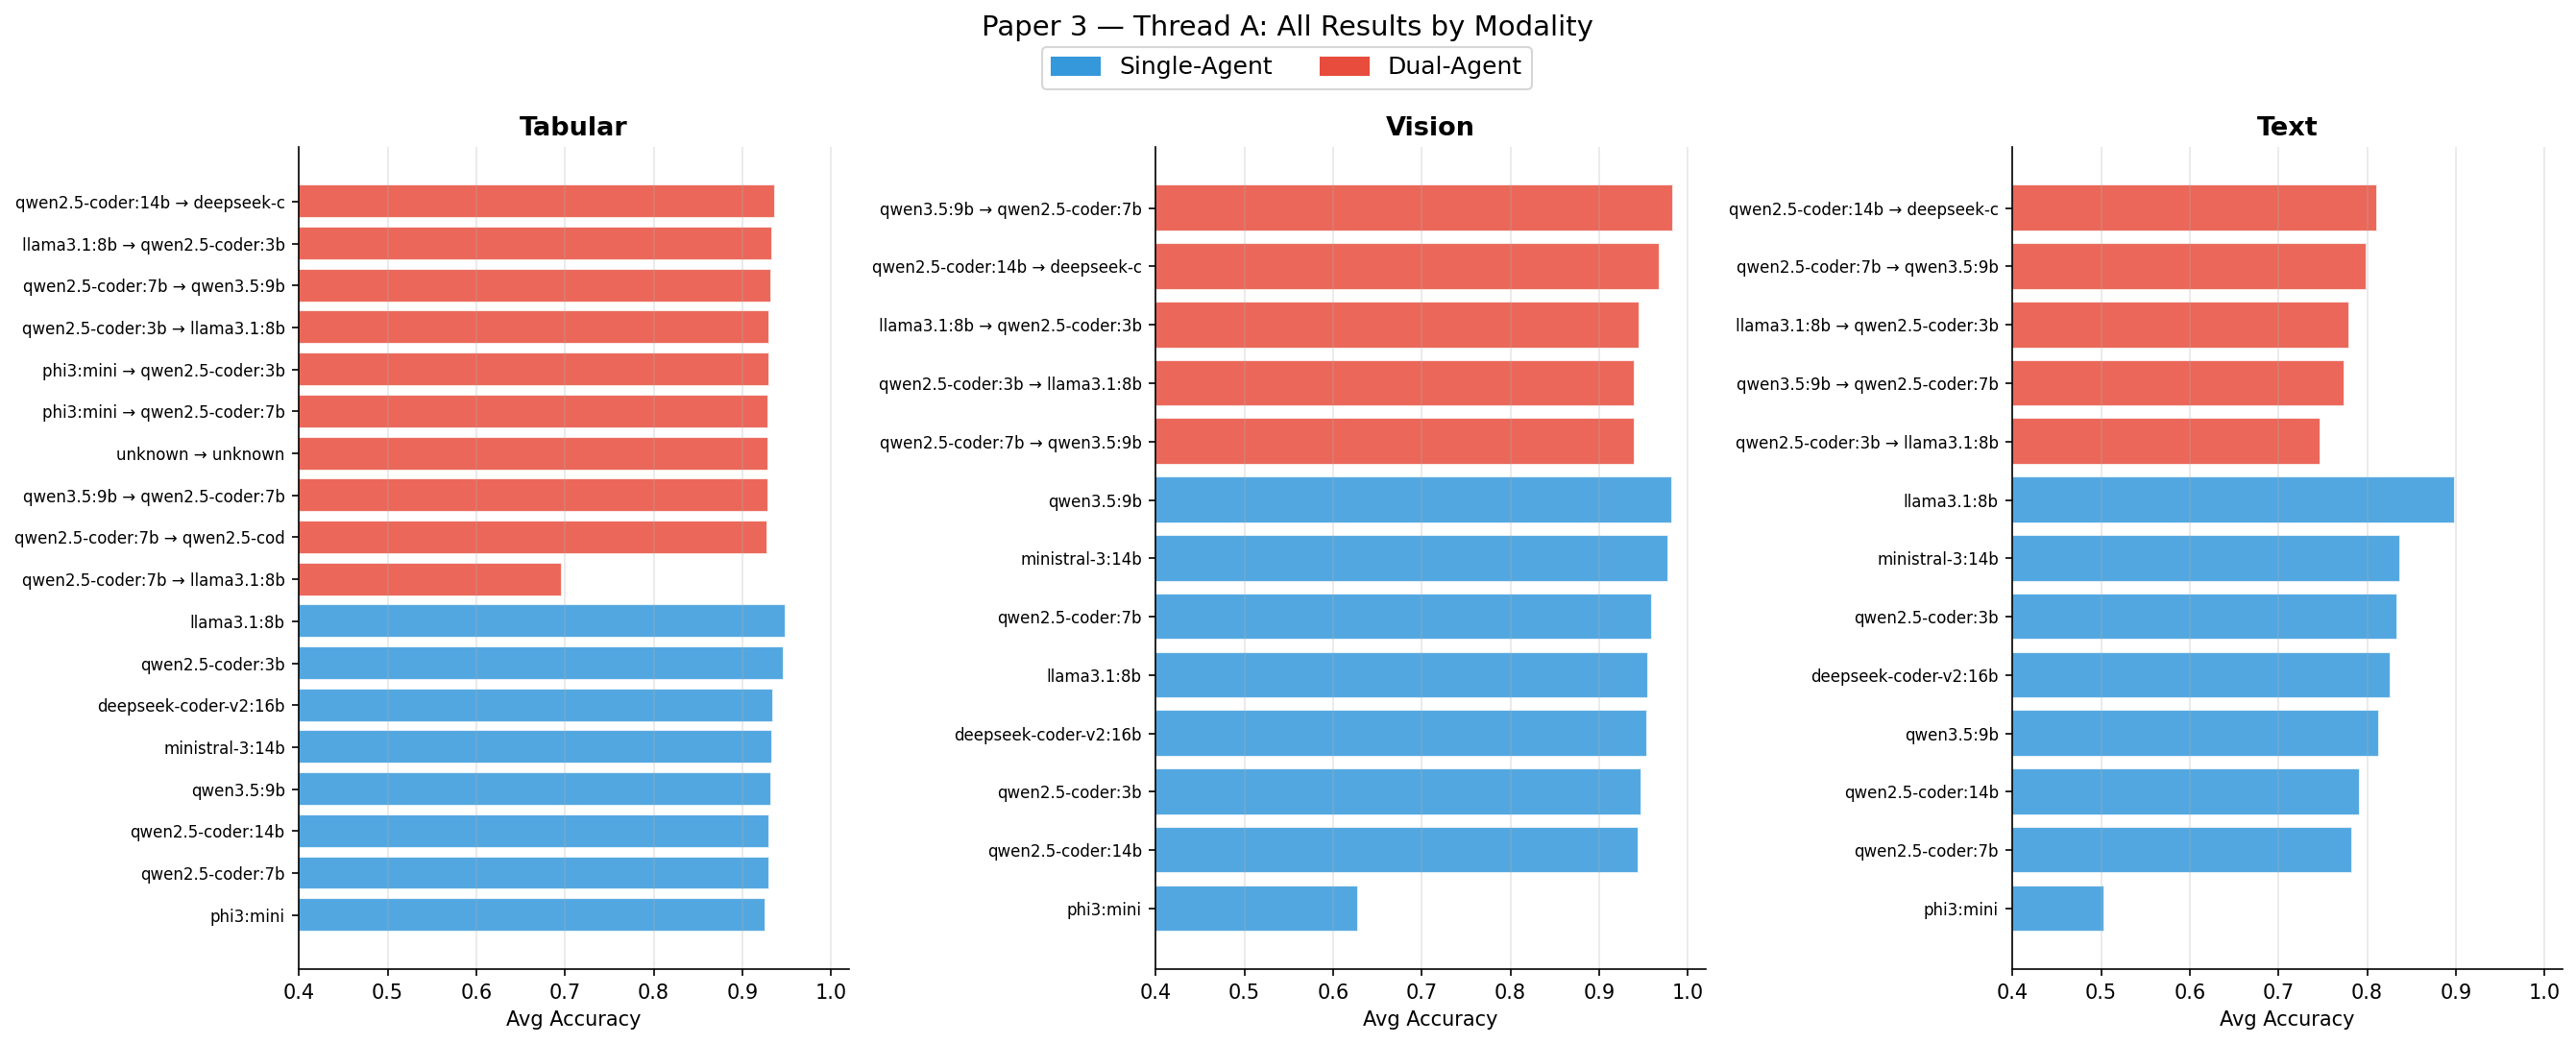
\includegraphics[width=0.95\textwidth]{figures/fig2_full_comparison.png}
    \caption{Full cross-modality leaderboard from \texttt{paper3\_thread\_a}. Blue bars are single-agent settings; red bars are dual-agent settings. Each bar is labeled with the evaluated model or reviewer$\rightarrow$coder pair.}
    \label{fig:full_comparison}
\end{figure}

This paper delivers empirical evidence that asymmetric \textbf{Agent-Critic (Reviewer-Coder)} loops improve stopping behavior under autonomous ML optimization. We concentrate on the Sunk-Cost mechanism, modality-specific dynamics, and mathematical halting boundaries.

Our contributions are:
\begin{enumerate}
    \item We formalize the \textbf{Autonomous Sunk-Cost Fallacy} in AEOS loops through explicit metrics: Sunk-Cost Episodes (SCE) and CADS.
    \item We evaluate single, dual, and tri-agent topologies across three ML modalities (Tabular, Text, Vision) using $N=132$ behavioral runs.
    \item We introduce and test an auditable mathematical halting intervention ($\Omega$ Cognitive Yield Engine) with a dedicated ablation of $N=36$ runs.
    \item We identify boundary conditions, including the modality paradox and Tri-Agent indecision behavior, and report both positive and negative outcomes.
\end{enumerate}

\textbf{Paper organization.} Section 2 positions this work against AutoML and agentic-loop literature. Section 3 defines methodology, formal metrics, architecture protocols, and prompting controls. Section 4 reports empirical results and research-question answers. Section 5 discusses the findings and practitioner implications. Sections 6--9 cover limitations, scope and future extensions, reproducibility notes, and conclusion.

\section{Related Work}

\textbf{AutoML and optimization loops.} Prior AutoML systems such as Auto-WEKA (Thornton et al., 2013), auto-sklearn (Feurer et al., 2015), and TPOT (Olson and Moore, 2016) established strong pipeline search and hyperparameter optimization paradigms. However, their primary framing is search quality and final performance, not language-agent stopping behavior under open-ended code-generation loops.

\textbf{LLM agent orchestration.} Multi-agent coding systems (e.g., MetaGPT and SWE-agent) show that role decomposition can improve execution quality and tool usage. Our setting differs in objective: we measure \textit{termination quality} and sunk-cost dynamics over long-horizon autonomous iterations, rather than task pass@k alone.

\textbf{Evaluator reliability.} Constitutional self-critique approaches (Bai et al., 2022) and LLM-as-judge evaluations (Zheng et al., 2023) motivate auditable oversight layers. This work extends that direction with an equation-level gate for halting decisions and with measurements of where reviewer policies fail without that gate.

\section{Methodology \& Formal Definitions}

\subsection{Sunk-Cost Episode (SCE)}

Let $A_t$ represent the best validation accuracy achieved up to iteration $t$. Let $M_t$ represent the machine learning model family deployed at iteration $t$. Let $D_t$ denote the directive emitted by the agent. A \textbf{Sunk-Cost Episode (SCE)} is a sequence of iterations $t \in [t_{\text{start}}, t_{\text{end}}]$ of length $L \ge 5$ where:
1. Zero Progress: $A_t - A_{t_{\text{start}}-1} < 0.001$
2. Strategy Anchoring: $M_t = M_{t_{\text{start}}}$
3. Halting Failure: $D_t \neq \text{"STOP"}$

\subsection{Cognitive Agentic Diversity Score (CADS)}

We categorize LLMs into foundational ``families'' (e.g., Qwen, LLaMA, DeepSeek, Gemma, Phi, Mistral). For an agentic panel $\mathcal{P}$ consisting of $k$ agents:
\begin{equation}
    \text{CADS}(\mathcal{P}) = |\{f_i \mid i \in \mathcal{P}\}|
\end{equation}
A Homogeneous Control has a CADS = 1, whereas Heterogeneous Pairings have CADS $\ge$ 2.

\subsection{The AEOS Multi-Agent Loop}

\begin{figure}[H]
    \centering
    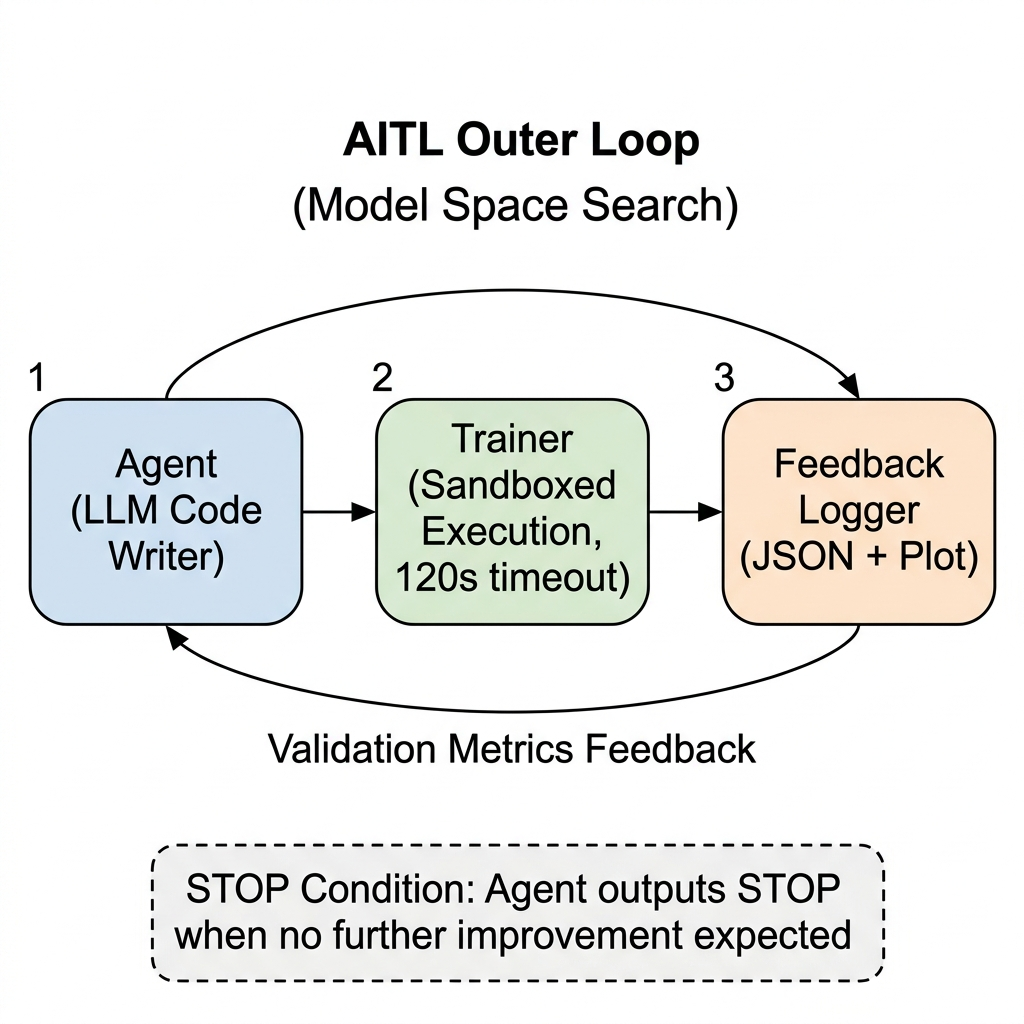
\includegraphics[width=0.9\textwidth]{figures/aeos_loop_diagram.png}
    \caption{The AEOS closed-loop orchestration cycle: Reviewer planning, sandboxed Coder execution, and mathematical $\Omega$ evaluation.}
    \label{fig:aeos_loop_diagram}
\end{figure}

The Reviewer inspects the history and outputs a high-level directive. The Coder receives the directive and writes a self-contained Python function. The code is executed in a sandboxed process. The Reviewer evaluates the new state and decides whether to continue iterating or stop.

\subsection{Execution Topologies in Paper 3}

\textbf{Single-Agent (Exp1):} one model serves as both strategist and coder. The same weight stack both plans and implements, so error-recovery and stopping judgment are self-referential.

\textbf{Dual-Agent (Exp2):} the Reviewer and Coder use different weights. The Reviewer emits only a directive; the Coder emits executable code. This creates a role boundary where strategic critique is decoupled from code generation.

\textbf{Tri-Agent (Exp3):} one Judge (Reviewer) and two parallel Coders run per iteration. Both coders receive the same directive, both candidate codes are executed, and only the better-performing candidate is written back into official history. This increases exploration pressure but can also create \textit{consensus drag}: the Judge keeps seeing ``some acceptable candidate'' and delays STOP.

\subsection{The \texorpdfstring{$\Omega$}{Omega} Cognitive Yield Stopping Engine}

To address the scenario where the LLM Reviewer fails to recognize a performance plateau, we wrap the loop in a mathematical optimization boundary called the \textbf{$\Omega$ Cognitive Yield Engine}. Operating on a sliding window of size $W=5$, it computes the cognitive yield $Y$:
\begin{equation}
    Y = \left(\frac{V}{W}\right) \times M
\end{equation}
where $V \in [0, W]$ is the number of successful iterations in the last window (non-error iterations with valid numeric metrics).

The progress multiplier $M$ is:
\begin{equation}
    M = \begin{cases}
        1.5 & \text{if } A_{\text{best}, k} - A_{\text{best}, k-1} > 0.001 \\
        0.1 & \text{if } V = 0 \text{ or } A_{\text{best}, k} - A_{\text{best}, k-1} < -0.005 \\
        0.5 & \text{otherwise}
    \end{cases}
\end{equation}

The decision boundary is:
\begin{equation}
    \text{Decision} = \begin{cases}
        \text{CONTINUE} & \text{if } Y \ge 0.5 \\
        \text{EXPLORE} & \text{if } 0.45 \le Y < 0.5 \\
        \text{STOP} & \text{if } Y < 0.45
    \end{cases}
\end{equation}

The engine injects its status dynamically into the Reviewer's system prompt to prevent reasoning drift.

\subsection{Reviewer System Prompts Used in Paper 3}

\textbf{Simple Reviewer Prompt (used in Exp1/Exp2/Exp3).} The core operational clauses are:
\begin{itemize}
    \item ``You CANNOT issue STOP before iteration 5 (minimum exploration floor).''
    \item ``You CANNOT issue STOP unless at least 3 DIFFERENT model families have been tried.''
    \item ``You SHOULD issue STOP when accuracy has not improved for 8+ consecutive successful iterations and 3+ families were tried.''
    \item ``Output exactly \texttt{DIRECTIVE: STOP} when halting is justified; otherwise output \texttt{DIRECTIVE: <one-sentence action>}.''
\end{itemize}

\textbf{Math Reviewer Prompt (used in \texttt{mathprompt} ablation).} The core operational clauses are:
\begin{itemize}
    \item Compute $V$ from the last 5 iterations, where \textbf{valid means non-error + numeric metric}. Timeouts, runtime failures, and sentinel rows are excluded.
    \item Compute $\Delta = A_{\text{best},k} - A_{\text{best},k-1}$, then set $M$ by the exact multiplier rule defined above.
    \item Compute $Y = (V/5)\times M$ and enforce: if $Y<0.45$, final line must be exactly \texttt{DIRECTIVE: STOP}.
    \item If $Y\ge0.45$, emit exactly one actionable instruction line for the Coder.
\end{itemize}

This section is intentionally explicit because Paper 3 evaluates stopping behavior; the prompt protocol is part of the intervention, not implementation noise.

\subsection{Experimental Setup and Controls}

\textbf{Datasets and splits.} All runs use AEOS standardized loaders and fixed train/validation splits for three modalities: Dry Bean (\texttt{tabular2}), 20 Newsgroups (\texttt{text}), and MNIST (\texttt{vision}).

\textbf{Run counts.} The baseline modality study aggregates $N=132$ runs across single, dual, and tri-agent configurations. The math-prompt study adds $N=36$ runs (3 datasets $\times$ 4 architectures $\times$ 3 repeats).

\textbf{Randomness policy.} The math-prompt ablation uses deterministic data seeds (seed start 42, repeated over 3 seeds). Core AEOS runs also use fixed seed-driven loading per run script; therefore, this paper emphasizes behavioral consistency and boundary detection over formal significance claims.

\textbf{Execution policy.} Each iteration executes generated code in a sandboxed subprocess with timeout caps, error capture, and explicit stop reasons (reviewer stop, safety cap, or forced stop on repeated failure).

\textbf{Metric reporting.} We report average accuracy, max accuracy, standard deviation, average iterations, SCE count, and wall-clock time in seconds. Time is interpreted as a systems-level operational metric, not a hardware-normalized benchmark.

\section{Empirical Results: Machine Learning Modalities}

We conducted $N=132$ experimental runs to evaluate single-agent models against asymmetric dual-agent pairings.

\subsection{Research Questions}

\textbf{RQ1.} Do asymmetric Reviewer$\rightarrow$Coder architectures reduce Sunk-Cost Episodes relative to single-agent loops?

\textbf{RQ2.} Does this behavior generalize across modalities (Tabular, Text, Vision), or is the optimum modality-dependent?

\textbf{RQ3.} What new failure modes emerge under tri-agent competitive generation?

\textbf{RQ4.} Can a mathematical self-reflection gate enforce reliable autonomous stopping without destroying peak accuracy?

\subsection{Statistical Reporting Note}

Most architecture rows use $n=3$ repeated runs, with some rows having additional historical reruns due to the iterative nature of the project. We therefore report descriptive uncertainty (mean, std, and full trajectory plots) and treat this paper as a behavioral systems study. Where needed, an approximate 95\% confidence interval can be read as:
\begin{equation}
    \mu \pm 1.96\frac{\sigma}{\sqrt{n}}
\end{equation}
but we avoid over-claiming significance in low-$n$ settings.

\subsection{Tabular Modality (\texttt{tabular2})}

\begin{table}[ht]
\centering
\footnotesize
\setlength{\tabcolsep}{3pt}
\caption{Tabular Single-Agent Leaderboard}
\label{tab:tabular_single}
\begin{adjustbox}{max width=\textwidth, center}
\begin{tabular}{>{\raggedright\arraybackslash}p{4.2cm}ccccccc}
\toprule
\textbf{Model} & \textbf{Runs} & \textbf{Avg Acc} & \textbf{Max Acc} & \textbf{Std Acc} & \textbf{Avg Iters} & \textbf{Avg SCE} & \textbf{Avg Time (s)} \\
\midrule
\textbf{llama3.1:8b} & 3 & 0.9492 & 0.9765 & 0.0194 & 103.7 & \textbf{8.7} & 3432.1 \\
qwen2.5-coder:3b$^\dagger$ & 4 & 0.9472 & 1.0000 & 0.0306 & 46.0 & 5.2 & 3430.5 \\
deepseek-coder-v2:16b & 7 & 0.9349 & 0.9385 & 0.0035 & 80.4 & \textbf{8.6} & 3996.9 \\
ministral-3:14b & 3 & 0.9338 & 0.9340 & 0.0002 & 63.7 & 4.3 & 5012.9 \\
qwen3.5:9b & 3 & 0.9323 & 0.9340 & 0.0017 & 65.3 & 5.3 & 6409.7 \\
qwen2.5-coder:14b & 7 & 0.9309 & 0.9390 & 0.0040 & 9.1 & 0.7 & 565.7 \\
qwen2.5-coder:7b & 4 & 0.9305 & 0.9390 & 0.0052 & 6.8 & 0.2 & 161.9 \\
phi3-mini & 4 & 0.9263 & 0.9305 & 0.0030 & 36.2 & 0.2 & 1172.0 \\
\bottomrule
\end{tabular}
\end{adjustbox}
\vspace{2pt}
\begin{minipage}{0.98\textwidth}
\footnotesize
$^\dagger$ Maximum accuracy of 1.0000 is likely an overfitting artifact on a small validation split. We keep the raw value for data integrity but do not treat it as representative capability.
\end{minipage}
\end{table}

\begin{table}[ht]
\centering
\footnotesize
\setlength{\tabcolsep}{3pt}
\caption{Tabular Dual-Agent Leaderboard}
\label{tab:tabular_dual}
\begin{adjustbox}{max width=\textwidth, center}
\begin{tabular}{>{\raggedright\arraybackslash}p{4.2cm}ccccccc}
\toprule
\textbf{Reviewer $\rightarrow$ Coder} & \textbf{Runs} & \textbf{Avg Acc} & \textbf{Max Acc} & \textbf{Std Acc} & \textbf{Avg Iters} & \textbf{Avg SCE} & \textbf{Avg Time (s)} \\
\midrule
\textbf{qwen2.5-coder:14b $\rightarrow$ deepseek-coder-v2:16b} & 3 & \textbf{0.9373} & 0.9395 & 0.0016 & 7.0 & \textbf{0.0} & 329.8 \\
llama3.1:8b $\rightarrow$ qwen2.5-coder:3b & 3 & 0.9332 & 0.9385 & 0.0038 & 16.3 & 0.0 & 422.9 \\
qwen2.5-coder:7b $\rightarrow$ qwen3.5:9b & 3 & 0.9325 & 0.9340 & 0.0021 & 11.3 & 0.0 & 703.9 \\
qwen2.5-coder:3b $\rightarrow$ llama3.1:8b & 3 & 0.9303 & 0.9320 & 0.0012 & 6.3 & 0.0 & 132.2 \\
phi3-mini $\rightarrow$ qwen2.5-coder:3b & 4 & 0.9303 & 0.9325 & 0.0013 & 13.0 & 0.8 & 395.4 \\
phi3-mini $\rightarrow$ qwen2.5-coder:7b & 4 & 0.9298 & 0.9340 & 0.0025 & 4.8 & 0.0 & 161.2 \\
qwen3.5:9b $\rightarrow$ qwen2.5-coder:7b & 3 & 0.9292 & 0.9295 & 0.0002 & 75.0 & \textbf{20.3} & 3427.2 \\
\midrule
\textit{qwen2.5-coder:7b $\rightarrow$ qwen2.5-coder:7b (control)} & 4 & 0.9281 & 0.9310 & 0.0023 & 6.5 & 0.0 & 301.8 \\
\midrule
qwen2.5-coder:7b $\rightarrow$ llama3.1:8b & 4 & 0.6967 & 0.9345 & 0.4023 & 4.2 & 0.0 & 293.0 \\
\bottomrule
\end{tabular}
\end{adjustbox}
\end{table}

\begin{figure}[H]
    \centering
    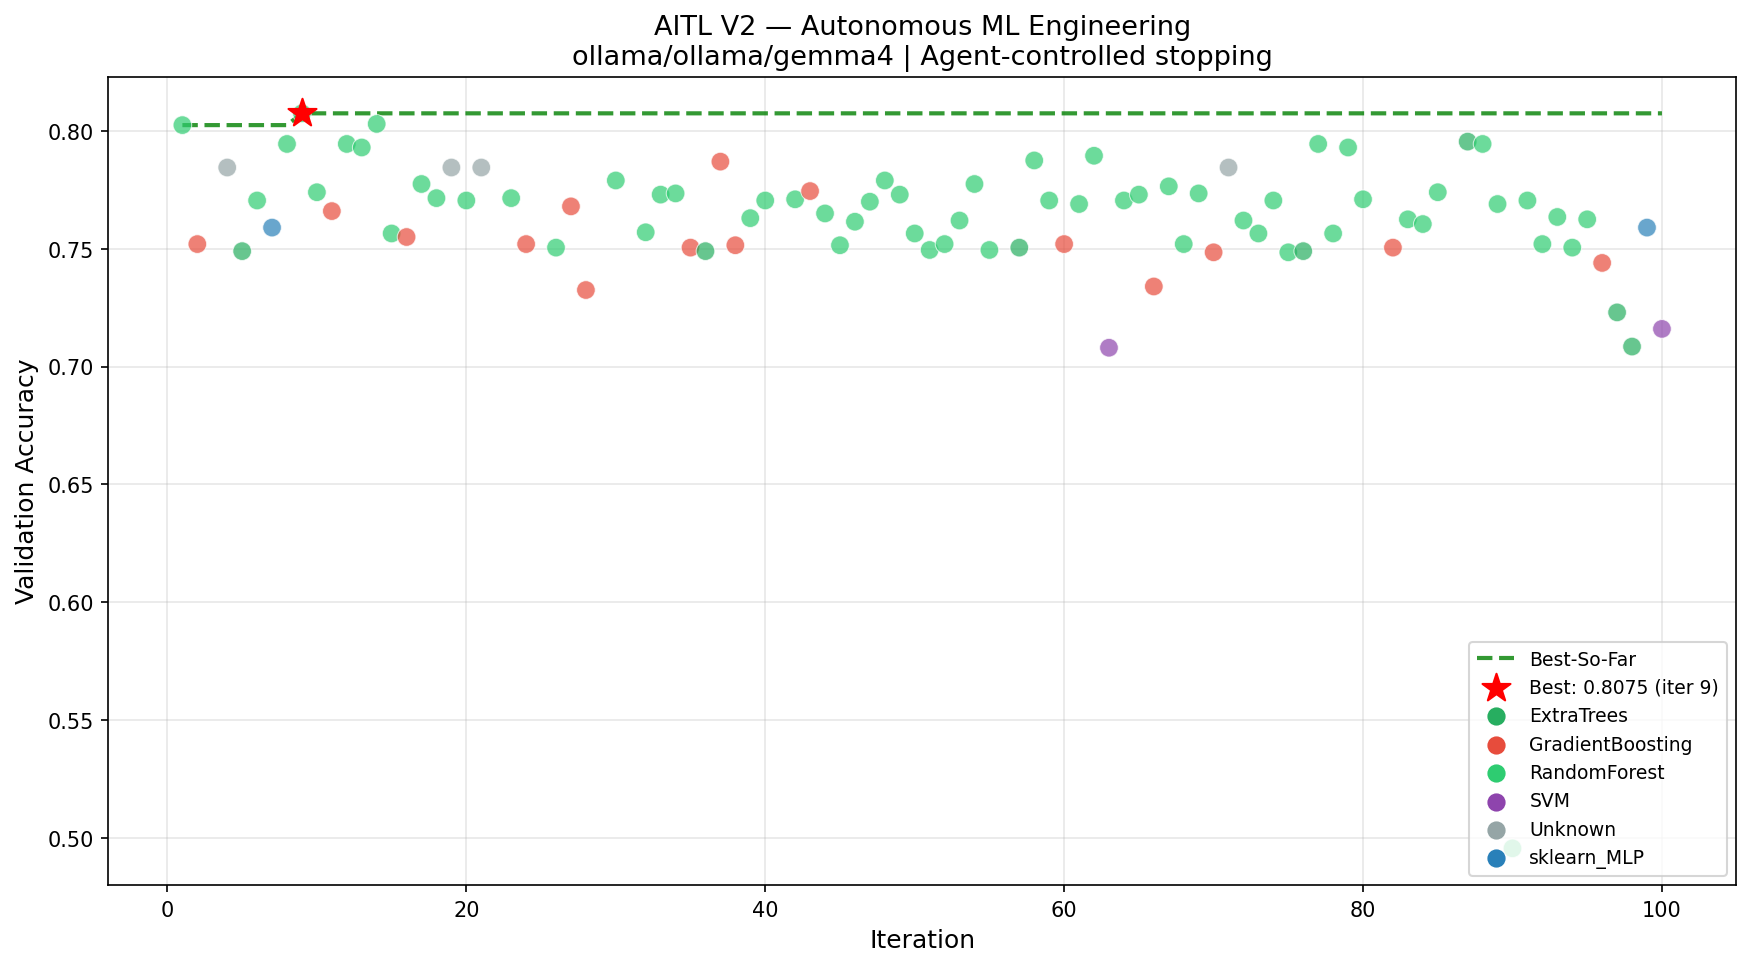
\includegraphics[width=0.8\textwidth]{figures/v2_plot_ollama_20260425_174014.png}
    \caption{Representative tabular trajectory showing a single model (\texttt{gemma4}) reaching peak accuracy at iteration 9, then continuing 91 additional low-yield iterations across 9 SCEs before hitting the safety cap.}
    \label{fig:tabular_trajectory}
\end{figure}

Under monolithic execution, general-purpose models like \texttt{llama3.1:8b} achieve high accuracies but suffer from massive strategic anchoring (averaging 8.7 SCEs). The asymmetric pairing \texttt{qwen2.5-coder:14b $\rightarrow$ deepseek-coder-v2:16b} achieves \textbf{98.7\% of the best single-agent accuracy in only 9.6\% of the execution time} (329.8s vs. 3432.1s). 7 of the 9 dual-agent configurations achieved exactly \textbf{0.0 SCEs}.

Two additional tabular findings are important for causal interpretation. First, the control ablation (\texttt{qwen2.5-coder:7b $\rightarrow$ qwen2.5-coder:7b}, CADS=1) averages 0.9281, while a heterogeneous pairing with the same reviewer family size (\texttt{qwen2.5-coder:7b $\rightarrow$ qwen3.5:9b}, CADS=2) reaches 0.9325 in its stronger runs, supporting a diversity benefit from weight asymmetry alone.

Second, not all asymmetry is beneficial. The pairing \texttt{qwen2.5-coder:7b $\rightarrow$ llama3.1:8b} has high variance (std 0.4023) and poor mean accuracy (0.6967), consistent with a reviewer that can stop quickly before coder recovery when initial code quality is unstable. Third, \texttt{qwen3.5:9b $\rightarrow$ qwen2.5-coder:7b} reaches the safety cap (75 iterations, 20.3 SCEs) on tabular data---a failure case that later in Section 4.4 becomes the positive counterexample in Vision, establishing the Modality Paradox as a true cross-task effect.


\subsection{Vision Modality (\texttt{MNIST})}

\begin{table}[ht]
\centering
\footnotesize
\setlength{\tabcolsep}{3pt}
\caption{Vision Single-Agent Leaderboard}
\label{tab:vision_single}
\begin{adjustbox}{max width=\textwidth, center}
\begin{tabular}{>{\raggedright\arraybackslash}p{4.2cm}ccccccc}
\toprule
\textbf{Model} & \textbf{Runs} & \textbf{Avg Acc} & \textbf{Max Acc} & \textbf{Std Acc} & \textbf{Avg Iters} & \textbf{Avg SCE} & \textbf{Avg Time (s)} \\
\midrule
\textbf{qwen3.5:9b} & 3 & 0.9827 & 0.9830 & 0.0002 & 25.0 & 0.0 & 2758.8 \\
ministral-3-14b & 3 & 0.9778 & 0.9815 & 0.0045 & 8.7 & 0.0 & 546.4 \\
qwen2.5-coder:7b & 3 & 0.9595 & 0.9645 & 0.0071 & 9.3 & 0.0 & 352.9 \\
llama3.1:8b & 3 & 0.9550 & 0.9670 & 0.0092 & 46.7 & 1.7 & 1847.3 \\
deepseek-coder-v2:16b & 3 & 0.9545 & 0.9570 & 0.0019 & 65.3 & \textbf{7.3} & 13763.5 \\
qwen2.5-coder:3b & 3 & 0.9480 & 0.9565 & 0.0060 & 61.3 & \textbf{9.0} & 4081.0 \\
qwen2.5-coder:14b & 3 & 0.9440 & 0.9495 & 0.0041 & 16.0 & 1.3 & 624.4 \\
phi3-mini & 3 & 0.6287 & 0.9475 & 0.4445 & 13.0 & 0.0 & 516.1 \\
\bottomrule
\end{tabular}
\end{adjustbox}
\end{table}

\begin{table}[ht]
\centering
\footnotesize
\setlength{\tabcolsep}{3pt}
\caption{Vision Dual-Agent Leaderboard}
\label{tab:vision_dual}
\begin{adjustbox}{max width=\textwidth, center}
\begin{tabular}{>{\raggedright\arraybackslash}p{4.2cm}ccccccc}
\toprule
\textbf{Reviewer $\rightarrow$ Coder} & \textbf{Runs} & \textbf{Avg Acc} & \textbf{Max Acc} & \textbf{Std Acc} & \textbf{Avg Iters} & \textbf{Avg SCE} & \textbf{Avg Time (s)} \\
\midrule
\textbf{qwen3.5:9b $\rightarrow$ qwen2.5-coder:7b} & 3 & \textbf{0.9840} & 0.9905 & 0.0085 & 75.0 & \textbf{10.3} & 6611.5 \\
qwen2.5-coder:14b $\rightarrow$ deepseek-coder-v2:16b & 3 & 0.9687 & 0.9795 & 0.0084 & 14.3 & 1.3 & 1319.4 \\
llama3.1:8b $\rightarrow$ qwen2.5-coder:3b & 3 & 0.9452 & 0.9495 & 0.0031 & 9.7 & 0.0 & 396.9 \\
\midrule
\textit{qwen2.5-coder:7b $\rightarrow$ qwen2.5-coder:7b (control)} & 1 & 0.9430 & 0.9430 & 0.0000 & 5.0 & 0.0 & 751.7 \\
\midrule
qwen2.5-coder:3b $\rightarrow$ llama3.1:8b & 3 & 0.9403 & 0.9430 & 0.0038 & 13.0 & 0.0 & 532.9 \\
qwen2.5-coder:7b $\rightarrow$ qwen3.5:9b & 3 & 0.9400 & 0.9430 & 0.0039 & 8.7 & 0.0 & 673.3 \\
\bottomrule
\end{tabular}
\end{adjustbox}
\end{table}

\textbf{The Modality Paradox:} In Tabular2, using \texttt{qwen3.5:9b} as Reviewer and \texttt{qwen2.5-\allowbreak coder:7b} as Coder is one of the least efficient configurations (75 iterations, 20.3 SCEs). In Vision, the same pairing becomes the top performer (avg 0.9840, max 0.9905). This inversion is the paper's strongest cross-modal systems finding: persistence that is harmful in shallow tabular search can be beneficial in high-dimensional visual optimization.

The mechanism is consistent with landscape shape. Vision training induces non-convex search trajectories where temporary regressions and long exploration windows can still produce later gains; therefore, reviewer ``stubbornness'' can act as productive persistence rather than waste. By contrast, more sensitive reviewers can stop too early in Vision: for example, \texttt{qwen2.5-coder:7b $\rightarrow$ qwen3.5:9b} halts around 8.7 iterations on average at 0.9400 accuracy. The operational conclusion is explicit: \textbf{task dimensionality dictates the optimal value of persistence}, so stopping policy should be modality-aware rather than globally fixed.


\subsection{Text Modality (\texttt{20 Newsgroups})}

\begin{table}[ht]
\centering
\footnotesize
\setlength{\tabcolsep}{3pt}
\caption{Text Single-Agent Leaderboard}
\label{tab:text_single}
\begin{adjustbox}{max width=\textwidth, center}
\begin{tabular}{>{\raggedright\arraybackslash}p{4.2cm}ccccccc}
\toprule
\textbf{Model} & \textbf{Runs} & \textbf{Avg Acc} & \textbf{Max Acc} & \textbf{Std Acc} & \textbf{Avg Iters} & \textbf{Avg SCE} & \textbf{Avg Time (s)} \\
\midrule
\textbf{llama3.1:8b} & 3 & \textbf{0.8988} & 0.9391 & 0.0531 & 113.3 & 1.7 & 3202.4 \\
ministral-3-14b & 3 & 0.8377 & 0.8379 & 0.0002 & 107.7 & 4.0 & 10381.1 \\
qwen2.5-coder:3b & 3 & 0.8344 & 0.8571 & 0.0161 & 50.3 & 8.0 & 1910.2 \\
deepseek-coder-v2:16b & 3 & 0.8265 & 0.8501 & 0.0329 & 129.3 & 7.7 & 7158.5 \\
qwen3.5-9b & 3 & 0.8129 & 0.8278 & 0.0166 & 79.3 & 1.3 & 11225.9 \\
qwen2.5-coder:14b & 3 & 0.7917 & 0.7980 & 0.0045 & 5.3 & 0.3 & 212.3 \\
qwen2.5-coder:7b & 3 & 0.7831 & 0.8067 & 0.0275 & 6.0 & 0.0 & 307.3 \\
phi3-mini & 3 & 0.5035 & 0.7739 & 0.3564 & 34.7 & 1.0 & 712.8 \\
\bottomrule
\end{tabular}
\end{adjustbox}
\end{table}

\begin{table}[ht]
\centering
\footnotesize
\setlength{\tabcolsep}{3pt}
\caption{Text Dual-Agent Leaderboard}
\label{tab:text_dual}
\begin{adjustbox}{max width=\textwidth, center}
\begin{tabular}{>{\raggedright\arraybackslash}p{4.2cm}ccccccc}
\toprule
\textbf{Reviewer $\rightarrow$ Coder} & \textbf{Runs} & \textbf{Avg Acc} & \textbf{Max Acc} & \textbf{Std Acc} & \textbf{Avg Iters} & \textbf{Avg SCE} & \textbf{Avg Time (s)} \\
\midrule
\textbf{qwen2.5-coder:14b $\rightarrow$ deepseek-coder-v2:16b} & 3 & \textbf{0.8116} & 0.8230 & 0.0161 & 8.7 & 0.0 & 596.5 \\
qwen2.5-coder:7b $\rightarrow$ qwen3.5:9b & 3 & 0.7996 & 0.8230 & 0.0207 & 14.3 & 0.0 & 1106.9 \\
llama3.1:8b $\rightarrow$ qwen2.5-coder:3b & 3 & 0.7802 & 0.8032 & 0.0163 & 10.0 & 0.0 & 625.6 \\
qwen3.5:9b $\rightarrow$ qwen2.5-coder:7b & 3 & 0.7744 & 0.8550 & 0.0573 & 75.0 & 17.3 & 4954.9 \\
qwen2.5-coder:3b $\rightarrow$ llama3.1:8b & 3 & 0.7476 & 0.7945 & 0.0332 & 9.7 & 0.0 & 598.4 \\
\bottomrule
\end{tabular}
\end{adjustbox}
\end{table}

Text shows the clearest boundary condition for naive asymmetry. The best single agent (\texttt{llama3.1:8b}, avg 0.8988, max 0.9391) outperforms all dual pairs in this dataset slice, while several dual systems trade away peak quality for faster termination. This contrasts with Tabular2 efficiency gains and indicates that ``dual is always better'' is empirically false.

A plausible mechanism is \textbf{sparse semantic gradient mismatch}. In 20 Newsgroups-style text classification, many incremental code changes do not produce smooth metric gains. Reviewer agents can interpret these flat or noisy intermediate steps as sunk-cost continuation and terminate before useful feature-pipeline recovery appears. The result is low-SCE but under-optimized runs: behaviorally well-stopped yet statistically suboptimal.

This is a boundary condition, not a contradiction. Single-agent \texttt{llama3.1:8b} requires long horizons (113.3 average iterations) and tolerates temporary stagnation before finding stronger configurations, while strong dual pairings terminate near 8--14 iterations. For sparse NLP regimes, the stopping logic likely needs semantic-progress signals beyond immediate validation deltas.


\begin{figure*}[ht]
    \centering
    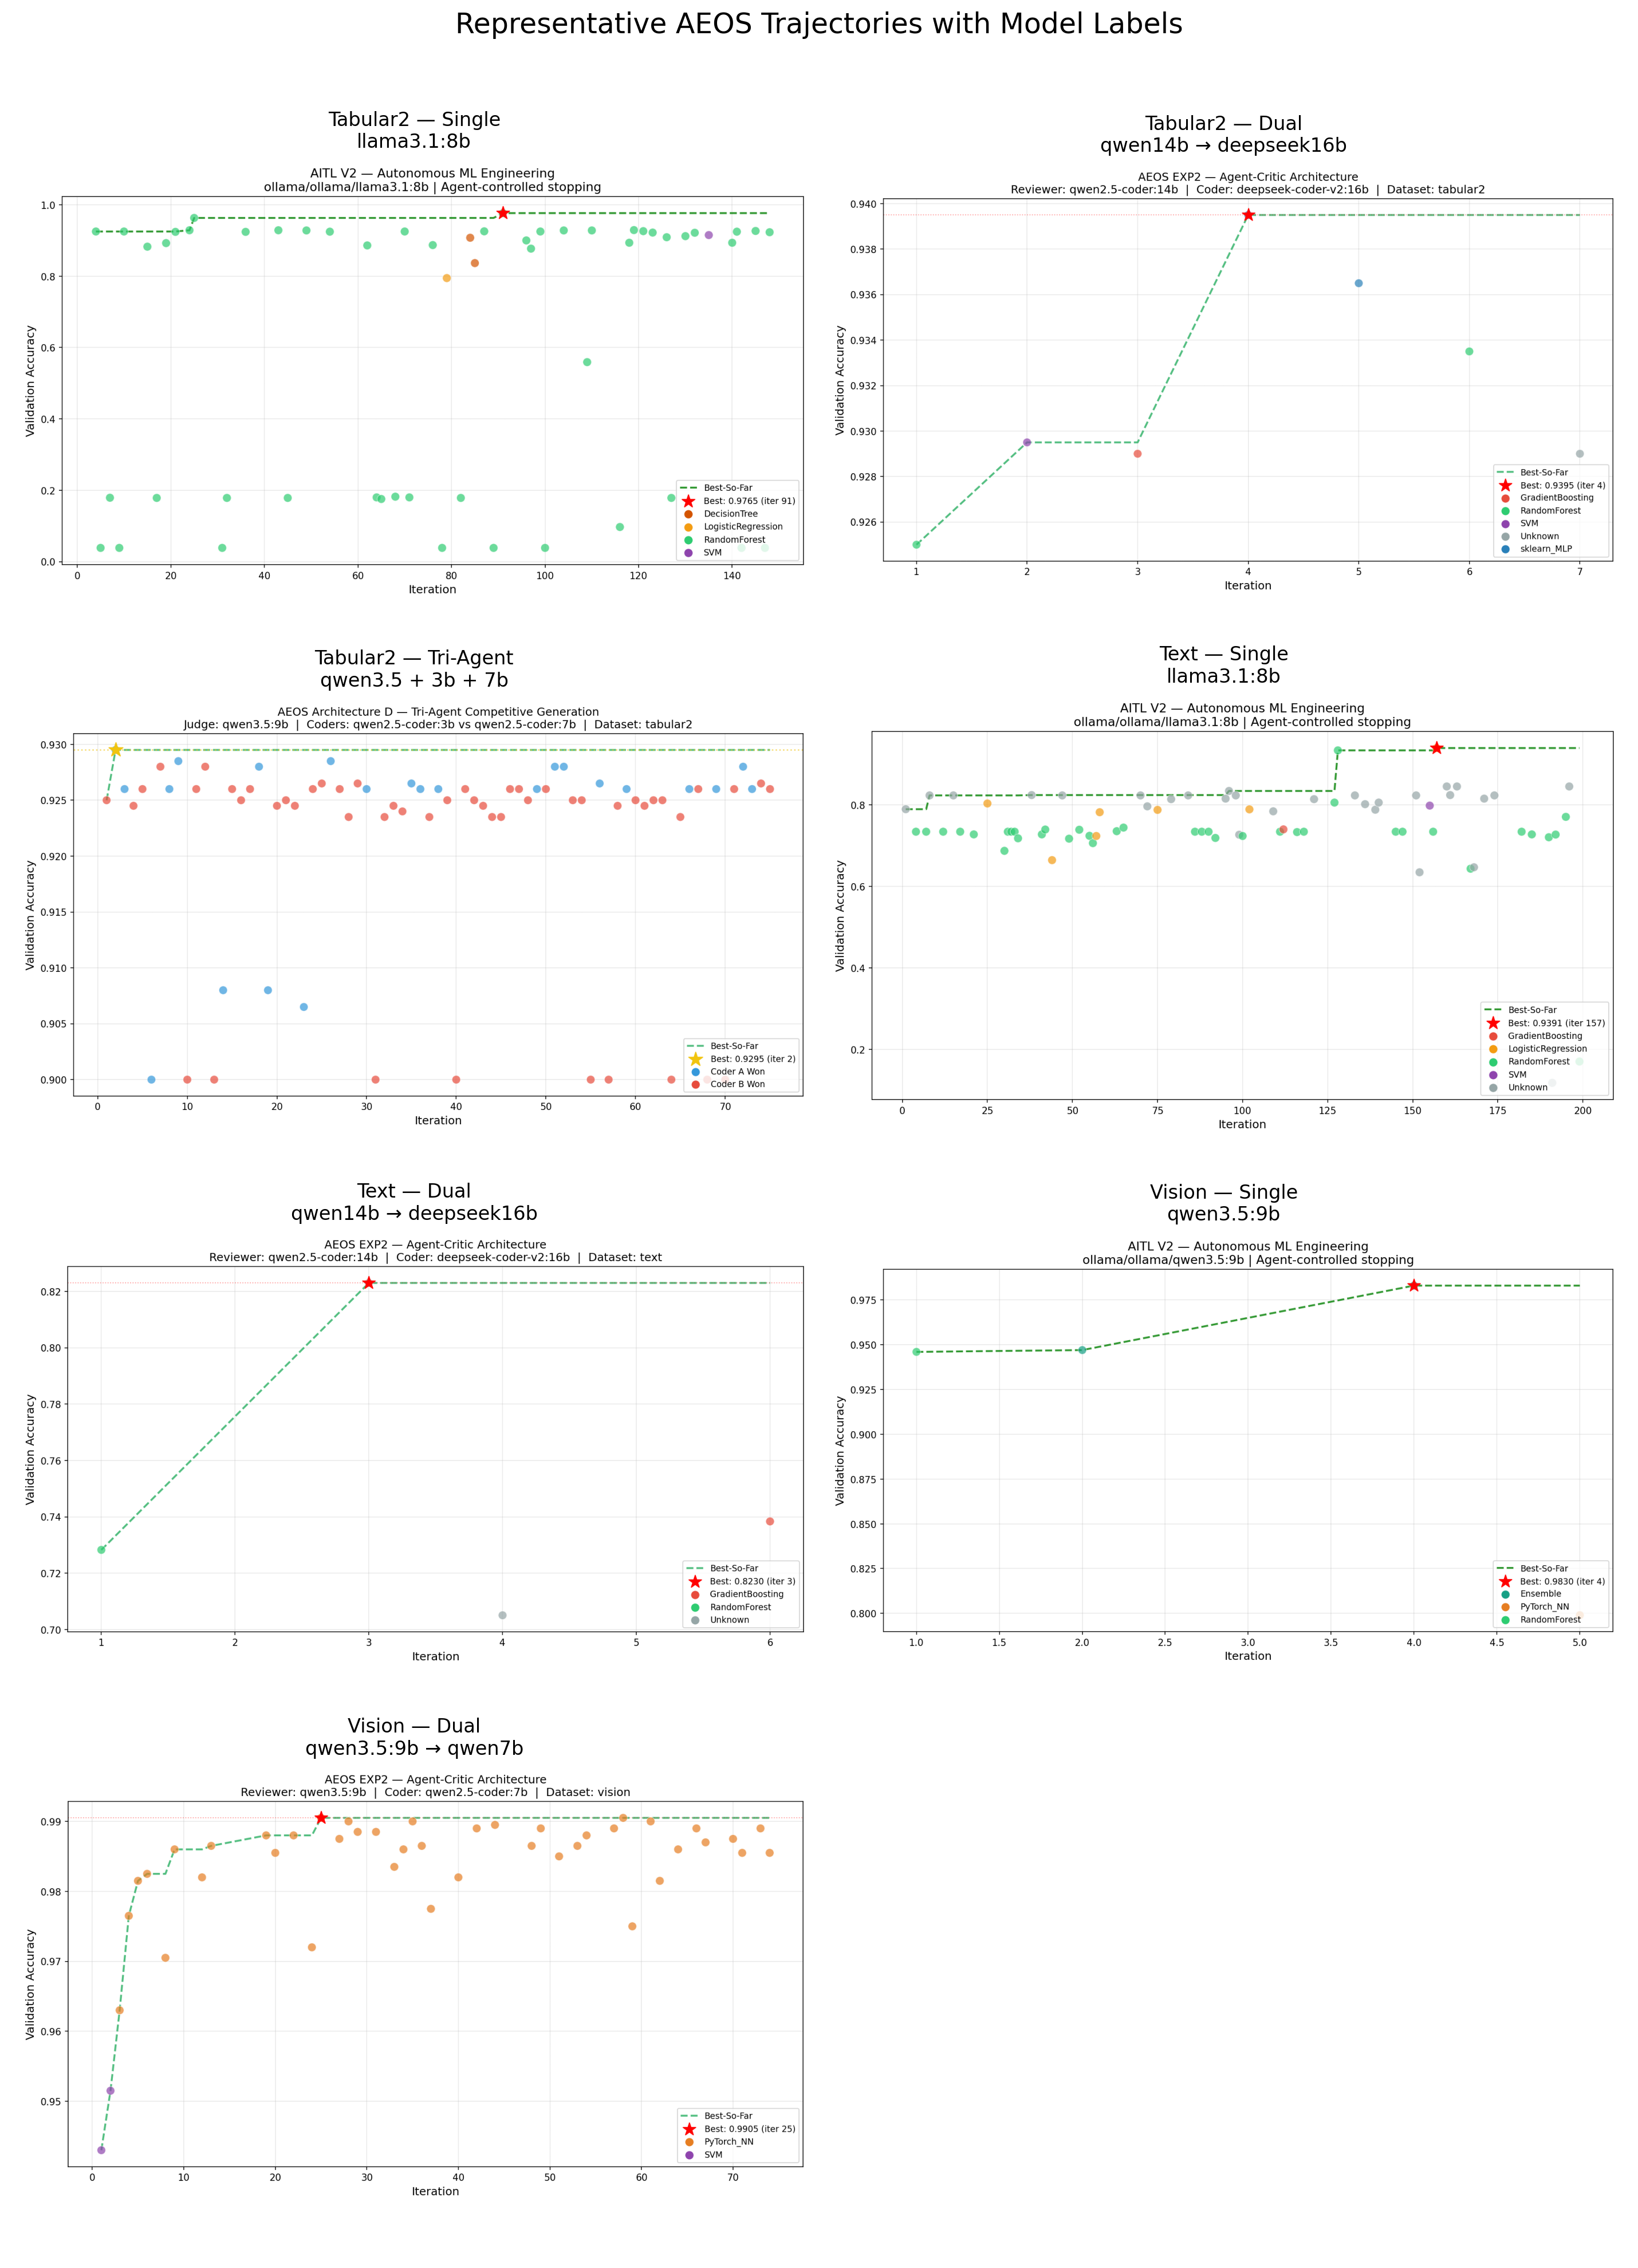
\includegraphics[width=\textwidth]{figures/fig3_representative_trajectories.png}
    \caption{Representative per-run trajectories combined from saved AEOS plots. Each panel shows modality plus the exact model (or reviewer$\rightarrow$coder pair) used in that run, giving a direct view of loop behavior behind the aggregate tables.}
    \label{fig:rep_trajectories}
\end{figure*}

\subsection{Tri-Agent Architecture and Cooperative Consensus}

\begin{table}[ht]
\centering
\footnotesize
\setlength{\tabcolsep}{3pt}
\caption{Tri-Agent Tabular Leaderboard}
\label{tab:tri_tabular}
\begin{adjustbox}{max width=\textwidth, center}
\begin{tabular}{>{\raggedright\arraybackslash}p{4.2cm}ccccccc}
\toprule
\textbf{Configuration} & \textbf{Runs} & \textbf{Avg Acc} & \textbf{Max Acc} & \textbf{Std Acc} & \textbf{Avg Iters} & \textbf{Avg SCE} & \textbf{Avg Time (s)} \\
\midrule
\textbf{qwen3.5:9b + 3b-coder + 7b-coder} & 3 & \textbf{0.9295} & 0.9295 & 0.0000 & 75.0 & 0.0 & 5680.4 \\
\bottomrule
\end{tabular}
\end{adjustbox}
\end{table}

\begin{figure}[ht]
    \centering
    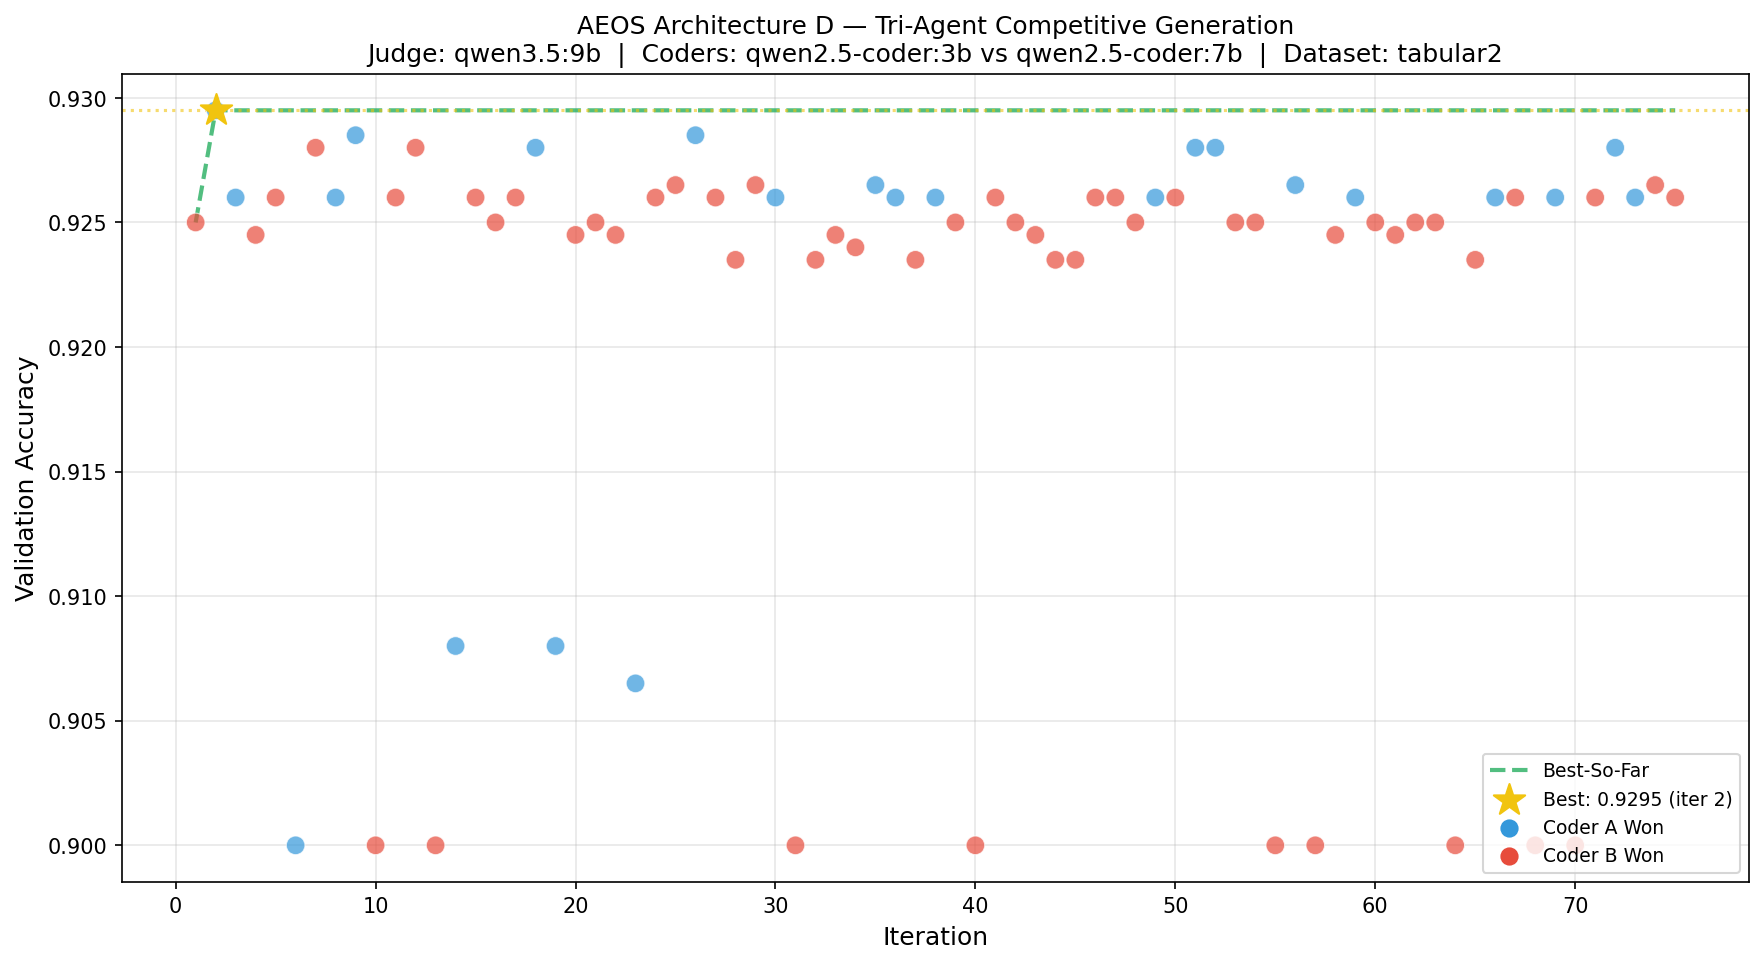
\includegraphics[width=0.9\textwidth]{figures/fig5_tri_loop_example.png}
    \caption{Representative Tri-Agent Tabular2 run. The Judge uses \texttt{qwen3.5:9b}; Coder A uses \texttt{qwen2.5-\allowbreak coder:3b}; Coder B uses \texttt{qwen2.5-\allowbreak coder:7b}. The run reaches the safety cap despite flat best accuracy.}
    \label{fig:tri_loop_example}
\end{figure}

Operationally, Exp3 uses a \textit{competitive writeback} mechanism: both coders execute in parallel, but only the better candidate is appended to the Judge's memory. This produces a strong local-selection bias---history contains the winner, not the full disagreement signal.

The Tri-Agent panel therefore reveals a distinct failure mode: the \textbf{Tri-Agent Indecision Loop}. Because the Judge repeatedly sees ``good enough'' alternatives and little explicit negative evidence, it delays \texttt{STOP} and can drift to safety-cap termination even when global best accuracy has already plateaued.

This failure mode is distinct from classical SCE continuation. In SCE-heavy single-agent behavior, one model repeatedly anchors on a narrow family with negligible gains. In Tri-Agent indecision, architectural variation can remain visible and SCE may appear low, yet the judge still overestimates exploration value because convergence between coders is not explicitly modeled. In all three tabular tri-agent runs, safety cap termination---not judge confidence collapse---ends the loop, motivating future consensus-decay signals for multi-coder panels.

\subsection{Mathematical Self-Reflection Ablation (\texttt{mathprompt}, N=36)}

\begin{table}[ht]
\centering
\footnotesize
\setlength{\tabcolsep}{3pt}
\caption{Math Prompt Ablation (N=36): Best Accuracy by Dataset and Architecture}
\label{tab:math_ablation}
\begin{adjustbox}{max width=\textwidth, center}
\begin{tabular}{>{\raggedright\arraybackslash}p{4.7cm}ccc}
\toprule
\textbf{Configuration} & \textbf{Tabular2} & \textbf{Text} & \textbf{Vision} \\
\midrule
SINGLE-llama3.1:8b-MATH & \textbf{0.9315 $\pm$ 0.0054} & 0.7984 $\pm$ 0.0083 & \textbf{0.9570 $\pm$ 0.0045} \\
DUAL-qwen14b$\rightarrow$deepseek16b-MATH & 0.9300 $\pm$ 0.0038 & \textbf{0.8200 $\pm$ 0.0272} & 0.9568 $\pm$ 0.0023 \\
SINGLE-qwen2.5-coder:7b-MATH & 0.9280 $\pm$ 0.0022 & 0.8136 $\pm$ 0.0271 & 0.9568 $\pm$ 0.0023 \\
DUAL-llama3.1:8b$\rightarrow$qwen2.5-coder:3b-MATH & 0.9297 $\pm$ 0.0038 & 0.8198 $\pm$ 0.0253 & 0.9423 $\pm$ 0.0272 \\
\bottomrule
\end{tabular}
\end{adjustbox}
\end{table}

\begin{figure}[ht]
    \centering
    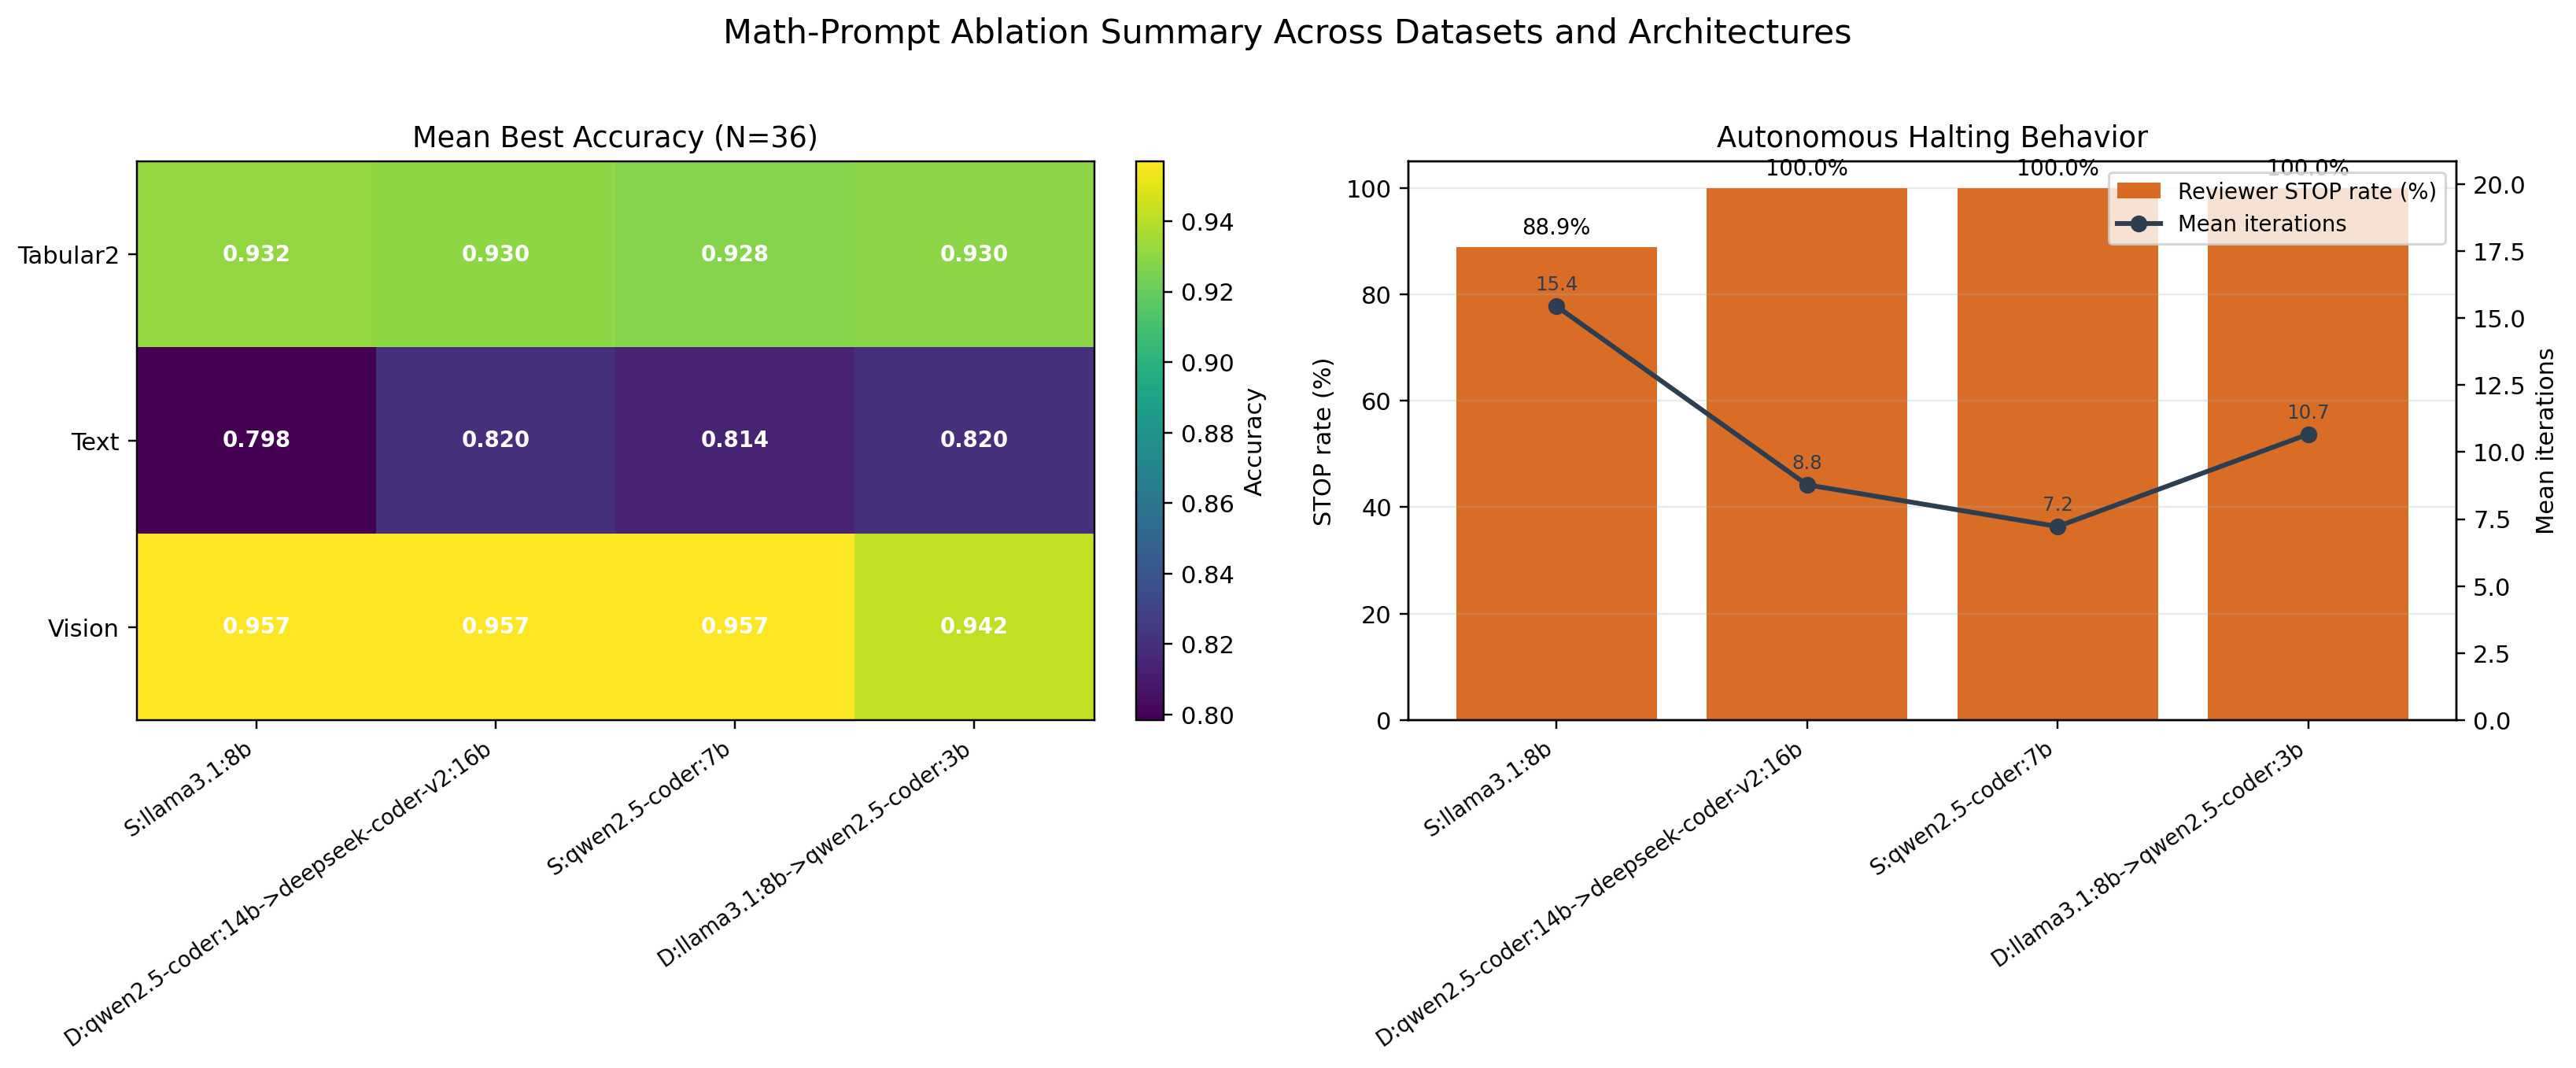
\includegraphics[width=\textwidth]{figures/fig4_mathprompt_ablation_summary.png}
    \caption{Math-prompt ablation summary from all 36 runs: (left) mean best accuracy by dataset and architecture; (right) reviewer STOP rate and mean iterations per architecture.}
    \label{fig:math_ablation_summary}
\end{figure}

Mechanistically, the halting decision is auditable at each iteration. Example from the dual Tabular2 run (\texttt{qwen14b$\rightarrow$deepseek16b}, iteration 9): $V=4$, $\Delta=0$, $M=0.5$, so $Y=(4/5)\times0.5=0.4<0.45$, which triggers an exact \texttt{DIRECTIVE: STOP}.

The mathematical self-reflection ablation confirms three key outcomes. First, autonomous halting remains strong: 35 of 36 runs ended with reviewer-issued STOP directives, with only one run reaching the hard safety cap. Second, the best architecture is modality dependent: single-agent \texttt{llama3.1:8b} leads Tabular2 and Vision, while the dual configuration using \texttt{qwen2.5-\allowbreak coder:14b} as Reviewer and \texttt{deepseek-\allowbreak coder-\allowbreak v2:16b} as Coder leads Text. Third, efficiency and peak accuracy diverge: in Tabular2 and Vision, near-tie accuracy can be achieved with materially lower runtime using smaller coder-weight configurations.

\section{Discussion}

\subsection{Interpretation of Key Findings}

RQ1 is supported in Tabular and Text by lower SCE counts in most asymmetric dual pairings than in strong single-agent baselines. RQ2 is also supported: architecture quality is modality-dependent, not globally ordered. The \textbf{Modality Paradox} is the key mechanism-level result---the same Reviewer$\rightarrow$Coder pair can be wasteful in one modality but productive in another.

RQ3 identifies a distinct tri-agent failure mode. Competitive dual-coder generation improves local candidate quality per step, but the judge can still delay halting when disagreement signals are weak in the persisted history (winner-only writeback). This creates indecision loops that safety caps, not reviewer judgment, terminate.

RQ4 is supported by the math ablation. The gate produces 35 reviewer-issued stops out of 36 runs while preserving near-tie best accuracy across architectures. This indicates that explicit, audited halting rules can stabilize loop termination without forcing a single universal architecture.

\subsection{Implications for Practitioners}

For autonomous ML engineering pipelines, the strongest actionable policy is: \textbf{fix the stopping rule, vary the topology by modality}. In practice, teams can use a conservative mathematical halting gate as a default safety layer, then choose single/dual/tri-agent structures based on dataset regime and search landscape complexity.

The second practitioner implication is operational: reporting only final accuracy is insufficient. Iteration counts, stop reasons, and SCE metrics reveal hidden compute waste and should be first-class dashboards in production autonomous loops.

A concrete default policy from this study is: prefer efficient single-agent code-tuned models for tabular regimes where short-horizon gains are common; permit higher-persistence reviewers for vision regimes where long non-convex exploration can still pay off; and treat sparse NLP regimes cautiously with dual-agent stopping thresholds, because low-SCE early stopping can undercut eventual quality.

\subsection{Theoretical Implications}

This study suggests there is no modality-agnostic notion of ``optimal persistence'' in autonomous LLM control loops. Persistence behaves as a task-conditioned control variable. Therefore, future adaptive-agent theory should model stopping as a function of both performance deltas and environment class, rather than as a static global threshold.

\section{Limitations}

\begin{itemize}
    \item \textbf{Statistical power:} many configurations use $n=3$ runs, which supports behavioral trend detection but limits strong significance claims.
    \item \textbf{Dataset breadth:} each modality is represented by one canonical dataset family in this paper; broader generalization remains open.
    \item \textbf{Time comparability:} wall-clock results are operationally useful but not hardware-normalized benchmarks.
    \item \textbf{Sandbox realism:} subprocess execution captures functional failures but is not a full containerized security model.
    \item \textbf{Model ecosystem scope:} results center on tested AEOS model families and may shift as model weights and inference stacks evolve.
\end{itemize}

\section{Scope and Future Extensions}

This manuscript is intentionally scoped to the Autonomous Sunk-Cost Fallacy in AEOS machine learning loops and mathematical halting behavior. The evaluation covers three ML modalities (Tabular, Text, Vision) with single, dual, and tri-agent architectures.

Two natural extensions are left to future work: (1) applying cognitive agentic diversity to unbounded logical reasoning tasks, where majority-voting consensus panels may substitute for the structured validation oracle that AEOS provides, and (2) transferring hybrid routing approaches to high-speed security classification, where specialist architectures may replace monolithic LLM judges for latency-critical threat detection. Both directions build directly on the stopping and diversity findings reported here.

\section{Reproducibility Notes}

Code, scripts, and run artifacts are available in the AEOS repository linked on the title page. Core reproduction commands are:
\begin{itemize}
    \item Baseline modality runs: scripts under \texttt{experiments/aeos/aeos\_behave/run\_*.ps1}
    \item Math ablation: \texttt{python run\_math\_ablation.py}
    \item Cross-modality aggregation: \texttt{python aggregate\_paper3.py}
    \item Paper figure refresh: \texttt{python build\_paper3\_assets.py}
\end{itemize}
We additionally persist per-iteration reviewer outputs, directives, errors, stop reasons, and trajectories in JSON for post-hoc verification.

\section{Conclusion}

Autonomous LLM engineering loops fail not only through poor model quality, but through poor termination behavior. Paper 3 formalizes this as the Autonomous Sunk-Cost Fallacy and evaluates it with explicit behavioral metrics.

Across $N=132$ baseline runs and a dedicated $N=36$ math-gated ablation, we find that asymmetric role separation plus equation-level stopping improves termination reliability, but architecture ranking is modality-dependent. Tri-agent systems add exploration power yet can introduce indecision loops without stronger halting discipline.

The broader systems claim is straightforward: reliable autonomy requires auditable stopping as a first-class design primitive. Future work should extend this framework to larger dataset suites, stronger statistical power, and hardware-normalized efficiency reporting.

\section{References}
\begin{itemize}
    \item Bai, Y., et al. (2022). ``Constitutional AI: Harmlessness from AI Feedback.'' \textit{arXiv preprint arXiv:2212.08073}.
    \item Chen, M., et al. (2021). ``Evaluating Large Language Models Trained on Code.'' \textit{arXiv preprint arXiv:2107.03374}.
    \item Feurer, M., et al. (2015). ``Efficient and Robust Automated Machine Learning.'' \textit{Advances in Neural Information Processing Systems}.
    \item Hong, S., et al. (2023). ``MetaGPT: Meta Programming for Multi-Agent Collaborative Framework.'' \textit{arXiv preprint arXiv:2308.00352}.
    \item Jajoo, S. (2026a). ``AI In The Loop (AITL): A Systems Taxonomy for Closed-Loop Autonomous Evaluation.'' \textit{Zenodo}. DOI: \texttt{10.5281/zenodo.19551173}. \url{https://zenodo.org/records/19551173}.
    \item Jajoo, S. (2026b). ``The Autonomous Sunk-Cost Fallacy: Stopping Failures and Meta-Reasoning in LLMs Deployed within AEOS.'' \textit{Zenodo}. DOI: \texttt{10.5281/zenodo.19846960}. \url{https://zenodo.org/records/19846960}.
    \item Olson, R. S., \& Moore, J. H. (2016). ``TPOT: A Tree-Based Pipeline Optimization Tool for Automating Machine Learning.'' \textit{Proceedings of the AutoML Workshop (PMLR)}.
    \item Thornton, C., Hutter, F., Hoos, H. H., \& Leyton-Brown, K. (2013). ``Auto-WEKA: Combined Selection and Hyperparameter Optimization of Classification Algorithms.'' \textit{KDD}.
    \item Yang, J., et al. (2024). ``SWE-agent: Agent-Computer Interfaces Enable Automated Software Engineering.'' \textit{arXiv preprint arXiv:2405.15793}.
    \item Zheng, L., et al. (2023). ``Judging LLM-as-a-Judge with MT-Bench and Chatbot Arena.'' \textit{arXiv preprint arXiv:2306.05685}.
\end{itemize}

\end{document}
